%%%%%%%%%%%%%%%%%%%%%%%%%%%%%%%%%%%%%%%%%
%%% HYPERRIDE Reporting Template
%%%%%%%%%%%%%%%%%%%%%%%%%%%%%%%%%%%%%%%%%

\documentclass[letterpaper,12pt]{report}
\usepackage[pass]{geometry}
%\documentclass[11pt]{report}

\usepackage{hyperride}		% HYPERRIDE specific definitions and styles  
\usepackage[utf8]{inputenc}	% UTF8 package
\usepackage[T1]{fontenc}
\usepackage{textcomp}		% common special chars
\usepackage{amsmath}		% math formula
\usepackage{fancybox}
\usepackage{anyfontsize}	% fonts
\usepackage{lipsum}
\usepackage{float}
\usepackage[normalem]{ulem}
\usepackage{cleveref}
\usepackage[printonlyused]{acronym}
\hypersetup{
	pdftitle={Beacon Network Security Labs: Android VenomAttack Lab},
	pdfauthor={[Gunnar Vittrup, Gaby Dagher]},
	pdfkeywords={Periodic Report, European Union (EU), H2020, Project, HYPERRIDE, GA 957788},
}
\usepackage{subfigure}
\usepackage{graphicx}
\usepackage{xcolor}
\usepackage{soul}
\sethlcolor{lightgray}
\usepackage[export]{adjustbox}
\usepackage{mdframed}
\usepackage{pdfpages}
\usepackage{comment}
\usepackage{multirow,array}
\def\todo#1{{\color{hyperridered}\textbf{TODO:} ``#1''}}
\def\hyperride{HYPERRIDE}

\graphicspath{ {graphics/} }

%%%%%%%%%%%%%%%%%%%%%%%%%%%%%%%%%%%%%%%%%
%%% Definitions
%%%%%%%%%%%%%%%%%%%%%%%%%%%%%%%%%%%%%%%%%



% CHANGE %'s below to make subsection headings visible/invisible in TOC
%\newcommand{\xsubsubsection}[1]{\subsection{#1}}
%\newcommand{\xsubsubsection}[1]{\subsubsection{#1}}

\begin{document}

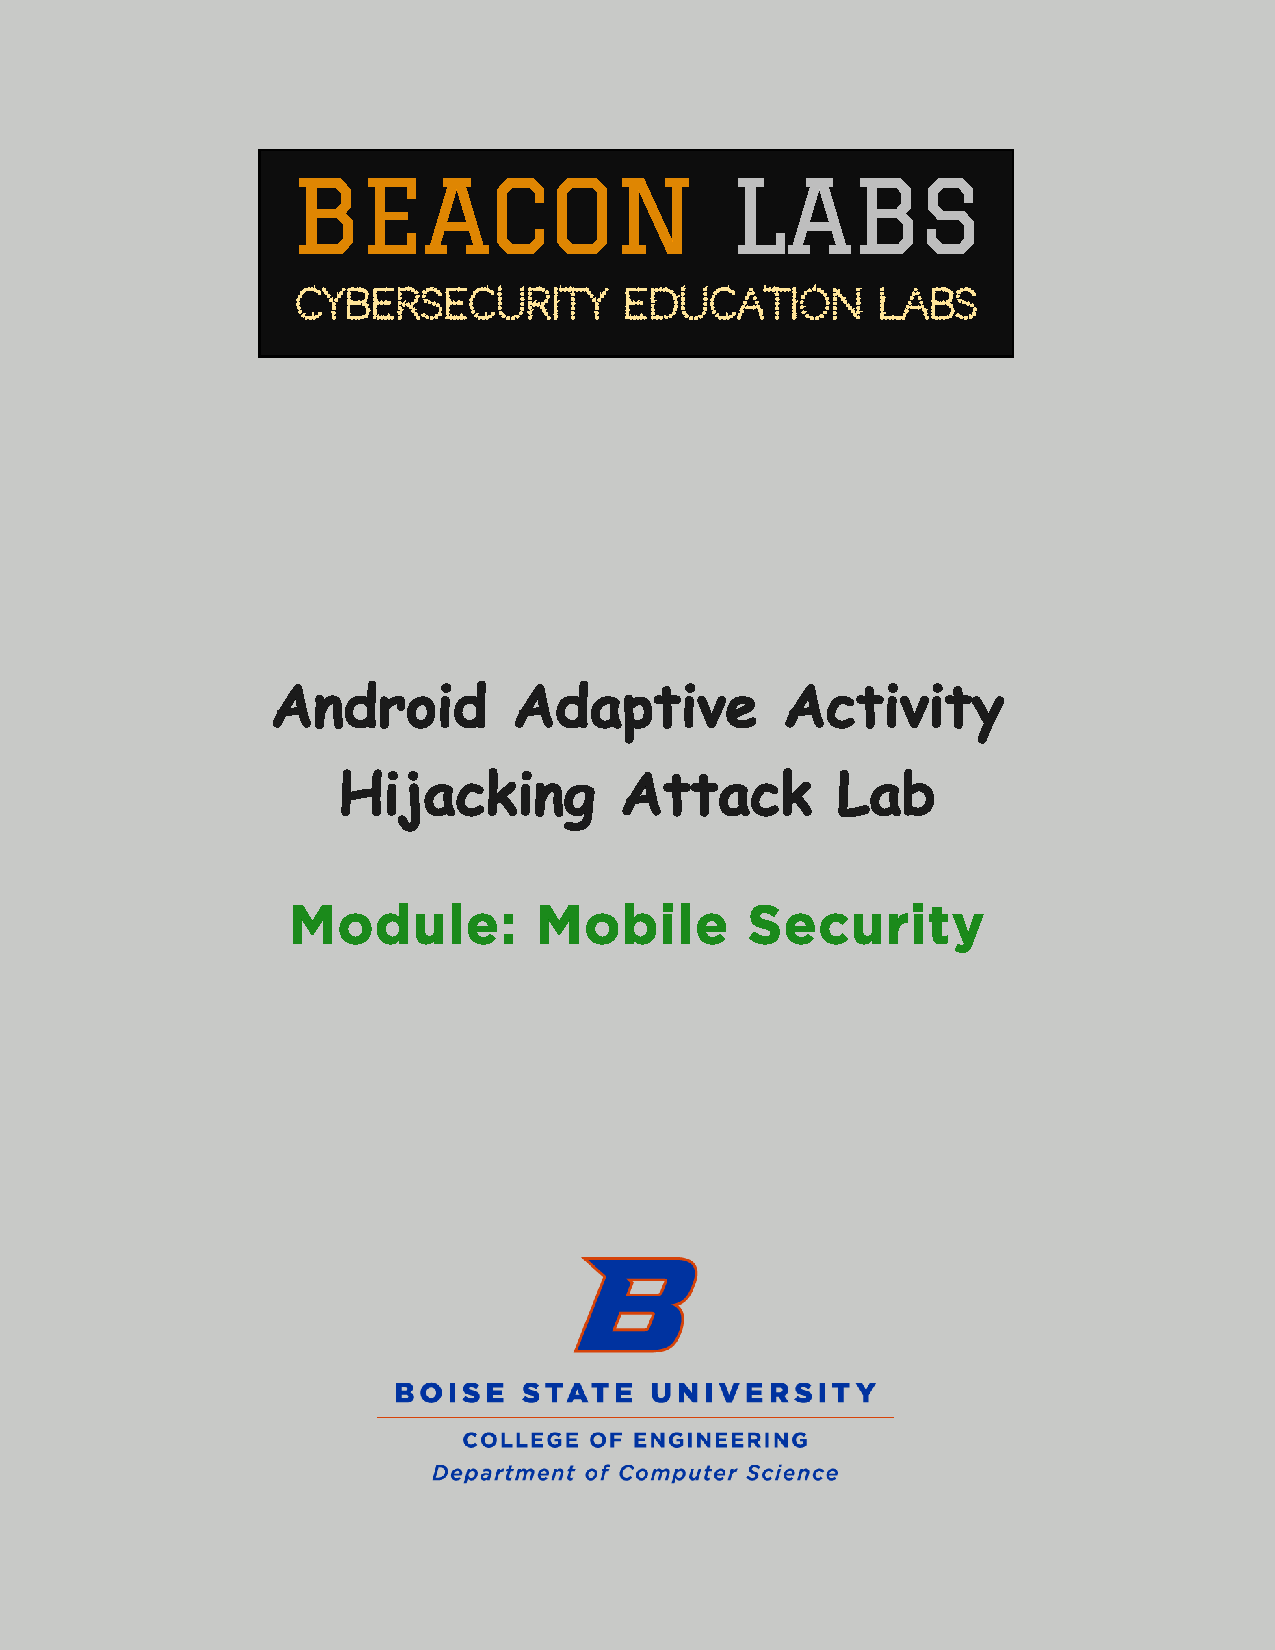
\includepdf[pages=1]{./graphics/FP-VenomAttack.pdf}

\mdfdefinestyle{code}{%
    linecolor=black,
    outerlinewidth=2pt,
    %roundcorner=20pt,
    innertopmargin=4pt,
    innerbottommargin=4pt,
    innerrightmargin=4pt,
    innerleftmargin=4pt,
        leftmargin = 4pt,
        rightmargin = 4pt
    backgroundcolor=black!10
    }

%%%%%%%%%%%%%%%%%%%%%%%%%%%%%%%%%%%%%%%%%
%%% URL style same as regular text
%%%%%%%%%%%%%%%%%%%%%%%%%%%%%%%%%%%%%%%%%
	
\urlstyle{same}

%%%%%%%%%%%%%%%%%%%%%%%%%%%%%%%%%%%%%%%%%
%%% Deliverable Information
%%%%%%%%%%%%%%%%%%%%%%%%%%%%%%%%%%%%%%%%%

% Project Meta Information
\ProjectFullTitle{Beacon Network Security Labs: Android VenomAttack Lab}
\ProjectAcronym{HYPERRIDE}
\ProjectRefNo{957788}

% Report Number, use either "1", "2", or "3" for the corresponding reporting period
\delivNumber{0}

% Period covered by the report
\delivFrom{dd/mm/yyyy}
\delivTo{dd/mm/yyyy}

% Report Responsible Partner
\delivResponsible{AIT Austrian Institute of Technology (AIT)} 

% Report Version, Contractual and Actual Date, Dissemination Level, Type
\delivVersion{vn.n}
\ContractualDate{dd/mm/yyyy}
\ActualDate{dd/mm/yyyy}

% List of Main Authors (usually from the responsible partner)
\delivAuthor{[Gunnar Vittrup, Gaby Dagher]}

% List of Co-Authors (all other co-authors should be listed here)
\delivFPAuthor{[]}

% Report Status
\delivStatus{d} %% d = draft, f = final, s = submitted

%%%%%%%%%%%%%%%%%%%%%%%%%%%%%%%%%%%%%%%%%
%%% Change Log
%%%%%%%%%%%%%%%%%%%%%%%%%%%%%%%%%%%%%%%%%

\istChange{dd/mm/yyyy}{v1.0}{Name (Partner short name)}{Draft report template}
\istChange{}{}{}{}

%%%%%%%%%%%%%%%%%%%%%%%%%%%%%%%%%%%%%%%%%
%%% Cover Page
%%%%%%%%%%%%%%%%%%%%%%%%%%%%%%%%%%%%%%%%%

%\makecover

%%%%%%%%%%%%%%%%%%%%%%%%%%%%%%%%%%%%%%%%%
%%% Table of Contents
%%%%%%%%%%%%%%%%%%%%%%%%%%%%%%%%%%%%%%%%%

\clearpage
\fancypagestyle{plain}{}
\settableofcontents
\tableofcontents
\clearpage

%%%%%%%%%%%%%%%%%%%%%%%%%%%%%%%%%%%%%%%%%
%%% Overview
%%%%%%%%%%%%%%%%%%%%%%%%%%%%%%%%%%%%%%%%%

\section*{Overview}\label{sec:work-carried-out}
\addcontentsline{toc}{section}{Overview}

Activity hijacking attacks were once one of the most powerful attacks against Android devices, but thanks to the presence of new effective defense mechanisms, they typically no longer pose security threats in more recent versions.

In this exercise, we explore a new state-of-the-art automated and adaptive hijacking attack that utilizes a spectrum of customized attacks. Specifically, we explore the use of hot patch techniques to identify vulnerable devices and update attack payload without the need for re-installation/re-distribution.

Furthermore, we'll utilize this service to receive a list of installed applications from the device via a remote server in order to determine a target application and recreate it utilizing an automated UI-generator tool known as Appium.

\subsection*{Objectives}

Upon completing this lab you should know how to connect an application to a remote server and returning device information in the background, utilize a hot patch framework to update application without need for re-installation, and generate automated UI tests with Appium.

\subsection*{Reading}

This lab is based on a paper by P. Sun, S. Chen, L. Fan, P. Gas, F. Song, and M. Yang,$^{[\text{\citeauthor{PSUN:171801}}]}$ and was published in the Frontiers of Computer Science. Reading the additional paper is not necessary but can help if you would like to learn more about this attack. 

${[\text{\citeauthor{PSUN:171801}}]}$ P. Sun, S. Chen, L. Fan, P. Gas, F. Song, and M. Yang, “VenomAttack: Automated and Adaptive Activity Hijacking in Android”, 2023.

%%%%%%%%%%%%%%%%%%%%%%%%%%%%%%%%%%%%%%%%%
%%% Setup
%%%%%%%%%%%%%%%%%%%%%%%%%%%%%%%%%%%%%%%%%

\section*{Setup}\label{sec:Setup}
\addcontentsline{toc}{section}{Setup}

A provided zipped folder contains all necessary files in order to run and complete this lab. It is recommended that you have 8 GB RAM or more, x86\_64 CPU architecture; 2nd generation Intel Core or newer, or AMD CPU with support for a Windows Hypervisor / ARM-based chips, or 2nd generation Intel Core or newer with support for Hypervisor.Framework, and 9 GB of available disk space minimum or more. 

\bigskip

Upon opening the provided lab folder in Android Studio, open a terminal into the topmost VenomAttack directory and run the command:

\bigskip
\begin{mdframed}[backgroundcolor=black!12,style=code,nobreak=true,align=center,userdefinedwidth=14cm]
    \$ git init
\end{mdframed}

The above command will initialize a new git repository which will be used in Action 2.3.2. You do not need to create a GitHub repository or commit your progress as you complete the lab.

First create your emulated device. On the right hand side of your screen, click the ‘Device Manager’ tab, and select ‘Create device’. Scroll down and select the ‘Pixel 5’ option. When choosing your system image, select the second tab that corresponds to your CPU architecture (x86 / ARM). Scroll down and select API 28 for Android 9 Pie. Make sure your application binary interface corresponds to your matching architecture. Lastly, make sure beneath the target column that your system image does not utilize Google API’s or services.

\bigskip

Now that you have created your device, run the device to confirm that it does so successfully. If any issues occur, refer to the appendix below or consult with Google. You will notice your device will be in a factory-stock state with the default applications installed. Navigate to your MainActivity class beneath the java application folder, right click it, and select “Run ‘MainActivity’”. This will cause the emulator to launch your device and install the application.  

\begin{figure}[!h]
    \centering
    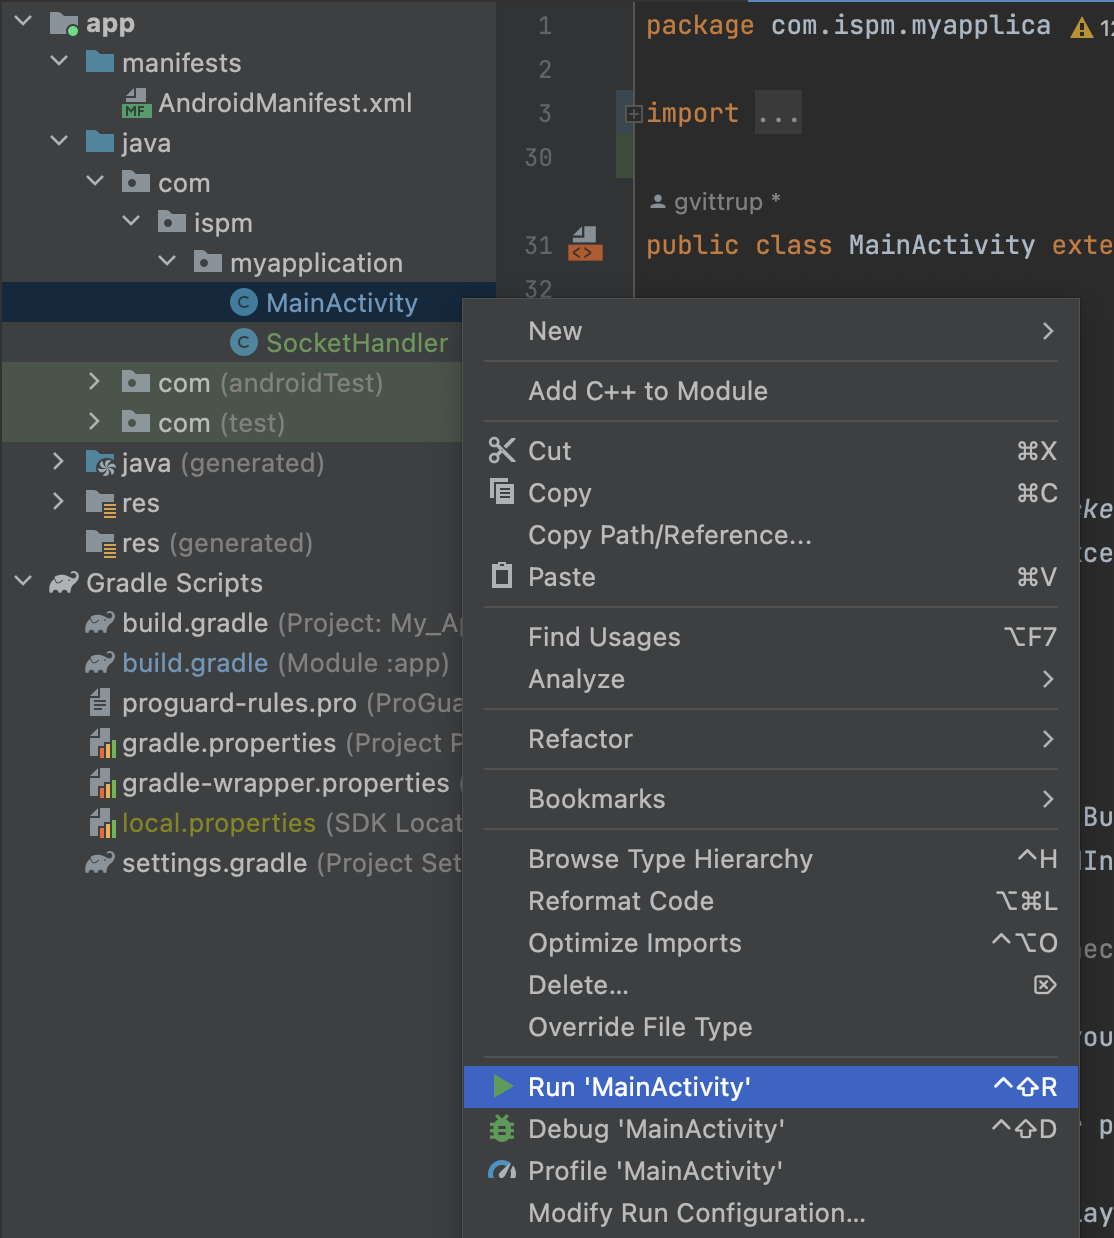
\includegraphics[scale=0.5]{graphics/run-ma.png}
    \caption{How to Compile MainActivity}
    \label{fig:run-ma}
\end{figure}

\bigskip

Next, install the latest version of \href{https://github.com/appium/appium-desktop}{Appium Server} on your respective device. Navigate to the link and locate the ‘Releases’ section on the right-hand side of the page. Below you will find a list of images beneath the ‘Assets’ tab. Appium Server allows you to connect to an emulated device via your system. 

\bigskip

Next, install the latest version of \href{https://github.com/appium/appium-inspector}{Appium Inspector} on your respective device. Navigate to the link and locate the ‘Releases’ section on the right-hand side of the page. Below you will find a list of images beneath the ‘Assets’ tab. Appium inspector allows you to attach to your Appium Server session and inspect a given device and activity.

\bigskip

Next, install the latest version of \href{https://nodejs.org/en}{Node.js}. Node.js is a runtime environment that allows us to host a server from our local machine. In this instance, we will use Node.js to host the remote server that our malicious activity connects to and sends information to. Navigate to the link and install the most recent LTS version of Node.js. To validate that you have successfully installed Node.js, you can run the command ‘node -v’ in your terminal which should output the version that you installed.

\bigskip

Lastly, it is required that you install the \href{https://developer.android.com/tools/adb}{Android Debug Bridge} (adb) in order to interact with your device from the command-line. Navigate to the link and make sure you have installed the SDK Manager and platform-tools that will allow you to utilize this command. To test this, run your device via Android Studio and then run the command `adb devices` to confirm that you see your device running on your machine.

\begin{figure}[!h]
    \centering
    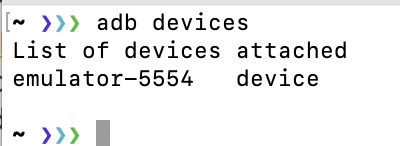
\includegraphics[scale=1.5]{graphics/adb-devices.png}
    \caption{Validating ADB Devices}
    \label{fig:adb-devices}
\end{figure}

%%%%%%%%%%%%%%%%%%%%%%%%%%%%%%%%%%%%%%%%%
%%% Lab Task 1
%%%%%%%%%%%%%%%%%%%%%%%%%%%%%%%%%%%%%%%%%

\section*{Task Set 1: Getting Device Information \& Sending it to a Remote Server}\label{sec:Task Set 1: Getting Device Information & Sending It To Remote Server}
\addcontentsline{toc}{section}{Task Set 1: Getting Device Information \& Sending it to a Remote Server}

\subsection*{Task 1.1: Getting Device Information}\label{sec:Task-1.1-Getting-Device-Information}
\addcontentsline{toc}{subsection}{Task 1.1: Getting Device Information}

The first step to this attack is to retrieve the information of the devices that your malicious activity is installed on. When a user opens your malicious application for the first time, your application will asynchronously send certain device information back to your remote server. This information being sent back contains two main components: a list of installed packages on the users device and the device resolution. The installed packages allow you to determine a target application that you can surmise a user will use on their target device. From here, you will take the target application and replicate it remotely within Android studio. The importance behind retrieving the resolution from the device is so you can match the native UI exactly. To do this successfully, you will use several built-in Android classes and functions. In order to get a list of packages, you can use the \href{https://developer.android.com/reference/android/content/pm/PackageManager}{PackageManager} class. The list can be retrieved using either the API function getInstalledPackages or the API function getInstalledApplications. The resolution can be achieved by utilizing the \href{https://developer.android.com/reference/android/util/DisplayMetrics}{DisplayMetrics} class. Retrieve this information utilizing the hints above and log this information to the Logcat console. When retrieving the device resolution, make sure that you are returning the \emph{real} resolution.

\emph{Note}: In order to log to the console, you will need to use Android’s Log function (Logcat), rather than Java’s console.log. 

\bigskip
\begin{mdframed}[backgroundcolor=blue!10,style=code,nobreak=true,align=center,userdefinedwidth=14cm]
\textbf{Action}
\bigskip

1.1.1 - Log to the console a list of installed packages along with the device resolution and submit a screenshot of both your output and your code.
\end{mdframed}

To go a step further, you can filter this list of packages to exclude any native system applications or services that would not be of interest to you as an attacker. This way, you would reduce the amount of network traffic being sent to and from the device, as well as reduce the amount of unnecessary information. This can be done in a multitude of ways.

\bigskip
\begin{mdframed}[backgroundcolor=blue!10,style=code,nobreak=true,align=center,userdefinedwidth=14cm]
\textbf{Action}
\bigskip

1.1.2 - What is one way you might be able to filter out some undesirable applications from the list of package names?
\end{mdframed}

\subsection*{Task 1.2: Creating the Remote Server}\label{sec:Task-1.2-Creating-the-Remote-Server}
\addcontentsline{toc}{subsection}{Task 1.2: Creating the Remote Server}

After successfully retrieving the device information within Android Studio’s console, the next step is to package it up and send the information to a remote server. For this, we will be using the java library socket.io. Socket.io allows us to use Node.js to host a server, create a socket, and connect to that endpoint from another program. Here, we will explore connecting our emulated device to this server when our malicious application is running. 

Follow the provided video part 1 on creating the Node.js server, titled "P1: Node.js Server."

\bigskip
\begin{mdframed}[backgroundcolor=blue!10,style=code,nobreak=true,align=center,userdefinedwidth=14cm]
\textbf{Action}
\bigskip

1.2.1 - Create an active Node.js server and connect to it via the localhost address in your browser. Submit a screenshot of the output of this page along with the output in your terminal logging what port your server is listening on.
\end{mdframed}

\subsection*{Task 1.3: Connecting and Communicating w/ the Remote Server}\label{sec:Task-1.3-Connecting-and-Communicating-w/-the-Remote-Server}
\addcontentsline{toc}{subsection}{Task 1.3: Connecting and Communicating w/ the Remote Server}

Now that you have successfully hosted your server on your local machine, its time to use socket.io to create a socket (or an endpoint) on the server for us to connect to from within our Android device.

Follow the second provided video tutorial, titled "P2: Socket.io," on how to set up and validate that your device is connecting. When done correctly, your server log should read that it has a new device connected.

\bigskip
\begin{mdframed}[backgroundcolor=blue!10,style=code,nobreak=true,align=center,userdefinedwidth=14cm]
\textbf{Action}
\bigskip

1.3.1 - Create an active connection to the remote server and submit a screenshot of your server log logging the new socket connection.
\end{mdframed}


\begin{figure}[!h]
    \centering
    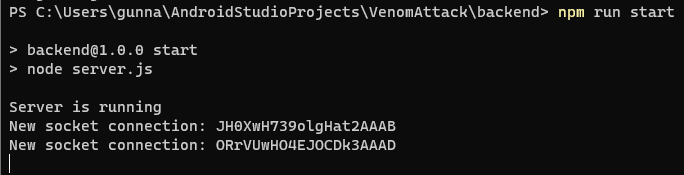
\includegraphics[scale=0.75]{graphics/socket-conn.png}
    \caption{Two Successful Socket Connections}
    \label{fig:socket-conn}
\end{figure}

After successfully connecting to the device, the next step is sending the information remotely. You may decide how you send this over. For the list of package names, you will want to send an array, and you can choose to either handle this on the server side or the client side. 

\bigskip
\begin{mdframed}[backgroundcolor=blue!10,style=code,nobreak=true,align=center,userdefinedwidth=14cm]
\textbf{Action}
\bigskip

1.3.2 - Send over the device information retrieved from your application, log it out to the console, and submit a screenshot that shows your socket connection, the real device resolution, and the list of package names.
\end{mdframed}


\begin{figure}[!h]
    \centering
    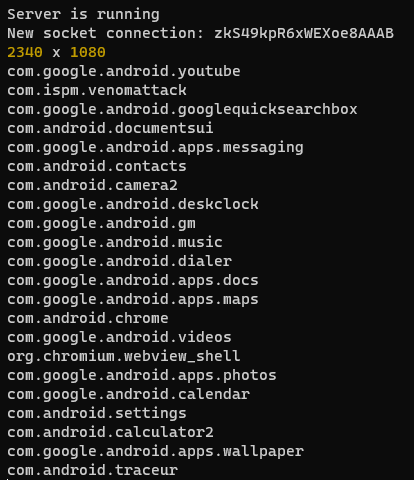
\includegraphics[scale=0.75]{graphics/device-info.png}
    \caption{Server Log of Device Information}
    \label{fig:device-info}
\end{figure}

%%%%%%%%%%%%%%%%%%%%%%%%%%%%%%%%%%%%%%%%%
%%% Task 2
%%%%%%%%%%%%%%%%%%%%%%%%%%%%%%%%%%%%%%%%%

\section*{Task Set 2: Recreating App w/ Appium and Creating Patchfile}\label{sec:Task Set 2: Recreating App w/ Appium and Creating Patchfile}
\addcontentsline{toc}{section}{Task Set 2: Recreating App w/ Appium and Creating Patchfile}

\subsection*{Task 2.1: Accessing Device via ADB Shell}\label{Task-2.1-Accessing-Device-via-ADB-Shell}
\addcontentsline{toc}{subsection}{Task 2.1: Accessing Device via ADB Shell}

By accessing the device via the ADB shell, you open the door to having much more control over the device you’re interacting with, most importantly being the developer tools. While the utility of the adb is incredibly extensive, our application will be rather simple.

In this particular instance, we will use it in order to retrieve the launch activity of a specific page of a desired application. In this phase of the attack, the idea is that the attacker has already retrieved device information remotely from an unsuspecting user. Now it is up to the attacker to mimic the application in order to create a fake activity that would steal user information. In many cases, in order to do this, the attacker will simply utilize an emulated device on their own machine. While in our context the emulated device will be the same device, the idea behind the process still stands.

In Android studio, make sure your emulated device is actively running. Within your terminal, run the command ‘adb devices’. You should see an output reading you the name of your emulator, as pictured in the setup section of this document. In order to run commands on this device, you will use the following command:

\bigskip
\begin{mdframed}[backgroundcolor=black!12,style=code,nobreak=true,align=center,userdefinedwidth=14cm]
    \$ adb -s <name\_of\_device>
\end{mdframed}
The -s flag allows us to specify the specific device you will be utilizing.

Running this command by itself will print out the version of the Android Debug Bridge you have along with the path where it is installed and a list of commands on how to use it. For example, to return a list of packages like we did in the first step, you can simply run the command:

\bigskip
\begin{mdframed}[backgroundcolor=black!12,style=code,nobreak=true,align=center,userdefinedwidth=14cm]
    \$ adb -s <name\_of\_device> shell pm list packages
\end{mdframed}

For the sake of this exercise, we will use the adb shell to retrieve the launch activity and package of a specific screen within our target application selected from the list of applications retrieved in the first step. 

For the target application itself, we recommend using the same target application used in the PHYjacking Lab, also by us. To use this application, download the project files for the PHYjacking Lab from \href{https://drive.google.com/file/d/1ACYQ1qE1wGhfaAeTw7Pt6uyXI6C_BEKZ/view?usp=share_link}{this Google Drive link}. Once downloaded, open up the project files and locate the AndroidManifest.xml file under PHYJacking-lab/app/src/main/ and changing the TransferPayActivity's exported attribute from false to true and then running the java file named "MainActivity.java" under the file path PHYJacking-lab/app/src/main/java/com/ispm/app/. This will install the app to the running emulation device.

In order to get the appropriate launch details with adb, navigate to the target application on your emulated device. In most attacks, the desired portion of an application in order to successfully perform a phishing attack is the login page. Navigate to the login page of the target application. Now, navigate back to your terminal and run the command as one line:

\bigskip
\begin{mdframed}[backgroundcolor=black!12,style=code,nobreak=true,align=center,userdefinedwidth=14cm]
    \$ adb shell "dumpsys window windows | grep -E \\  'mCurrentFocus|mFocusedApp'"
\end{mdframed}

This command will output the current focused app and activity on the emulated device, with the first portion of the output being the package name and the second portion being the launch activity. This information will be paramount to connecting to the application via Appium.

\bigskip
\begin{mdframed}[backgroundcolor=blue!10,style=code,nobreak=true,align=center,userdefinedwidth=14cm]
\textbf{Action}
\bigskip

2.1.1 - Retrieve the launch activity of the target application and the respective login page that you will utilize in the Appium server and submit a screenshot of your terminal output.
\end{mdframed}

\begin{figure}[!h]
    \centering
    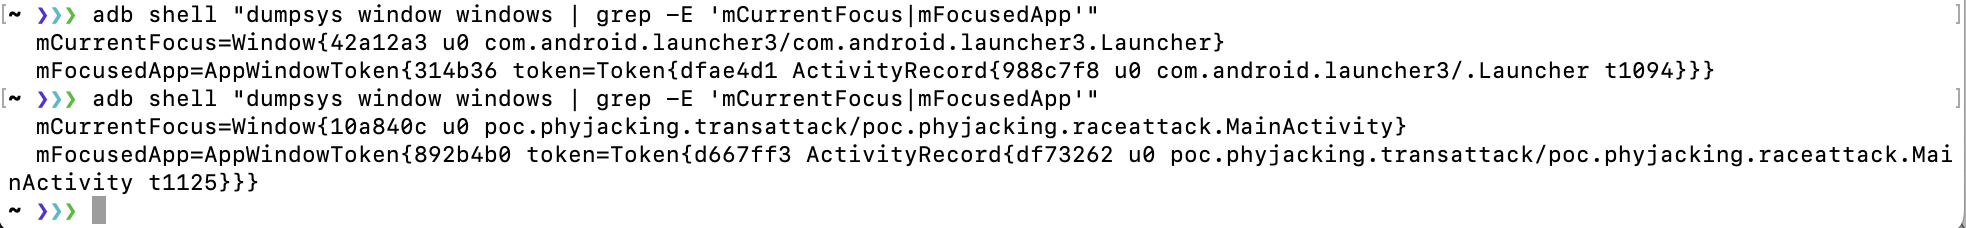
\includegraphics[scale=0.39]{graphics/adb-dumpsys.png}
    \caption{ADB Device Information}
    \label{fig:adb-dumpsys}
\end{figure}

\bigskip

\subsection*{Task 2.2: Connecting to Device Activity via Appium}\label{sec:Task-2.2-Connecting-to-Device-Activity-via-Appium}
\addcontentsline{toc}{subsection}{Task 2.2: Connecting to Device Activity via Appium}

From here, the next step requires us to take the information we garnered and input it into the Appium server. The information you’ve garnered in the previous exercises will be necessary to complete this next step. Load into the Appium Server GUI that you downloaded in the setup section of this document. You will be given two inputs: a host and a port. Set your host to “0.0.0.0” and your port number to an arbitrary and unused port. Then select “Start Server”. You should be provided with a terminal window from the Application that reads to you the server is running.

Now open the Appium Inspector tool. You will see a left hand set of parameters and a right-side JSON representation. In total, you will want to have 6 parameters that you pass to the server. These parameters will all be of type text and will read as follows:

\begin{enumerate}
    \item platformName: "android"
    \item platformVersion: "9"
    \item deviceName: "Pixel-5"
    \item automationName: "UiAutomator2"
    \item appPackage: ""
    \item appActivity: ""
\end{enumerate}

Where the last two parameters are provided by the information retrieved in the previous step. For the parameters at the top, set your Remote Host to “0.0.0.0”, the Remote Port to the port number you provided to the server, and your Remote Path to “/wd/hub/“. 

\begin{figure}[!h]
    \centering
    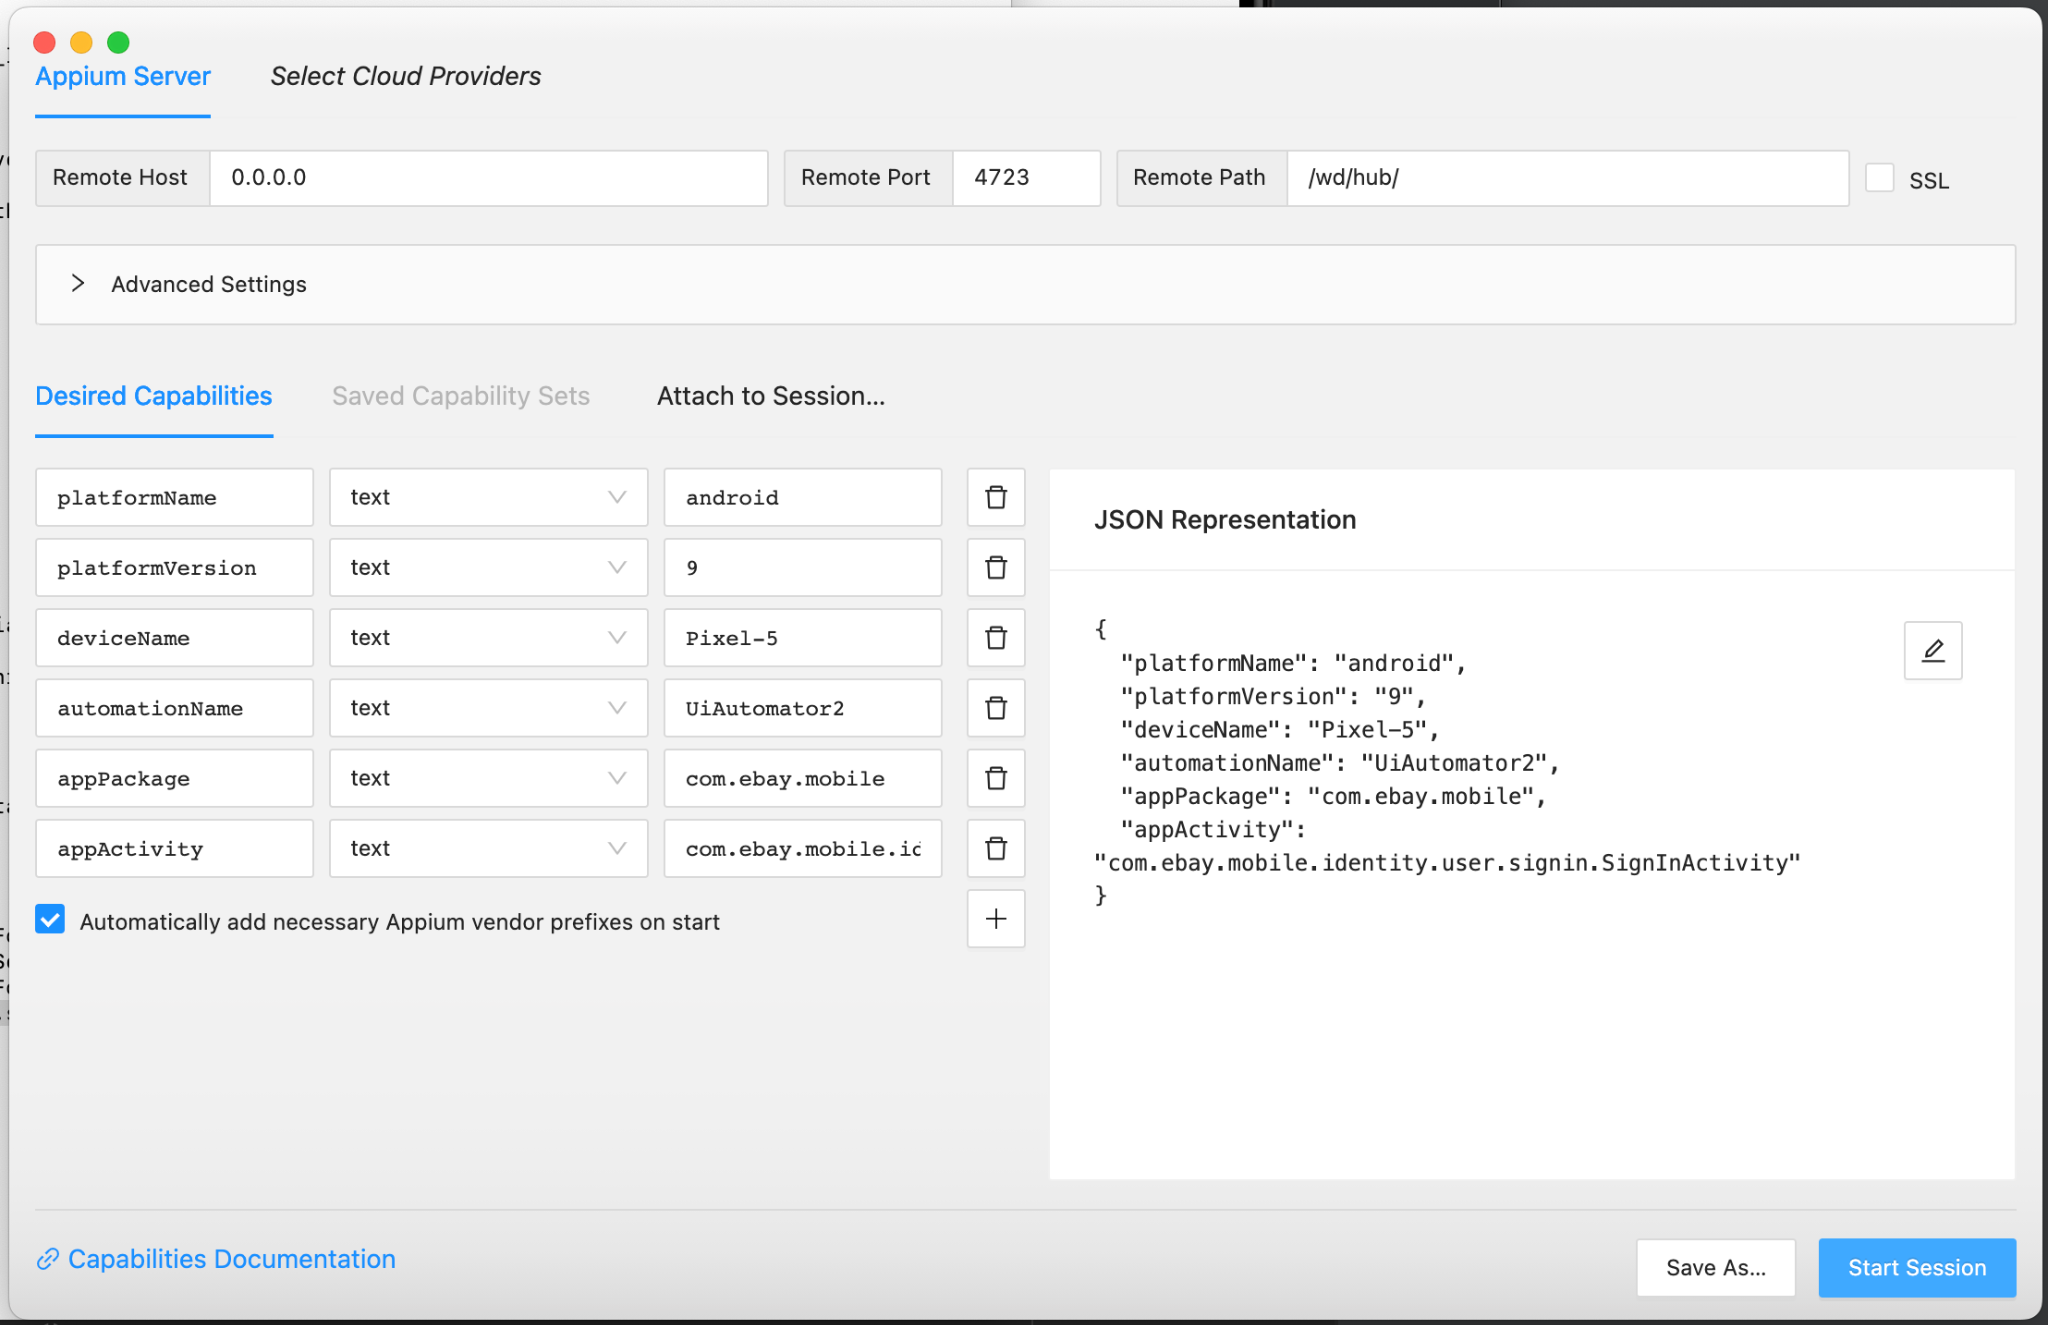
\includegraphics[scale=0.175]{graphics/appium-connection.png}
    \caption{Appium Connection Example}
    \label{fig:appium-connection}
\end{figure}

Once you have all these entered, select “Start Session”. If done so successfully, your Appium Server log should read to you the connection of your inspector with the parameters you passed, as noted in Figure~\ref{fig:appium-server} on page~\pageref{fig:appium-server}.

\begin{figure}[!h]
    \centering
    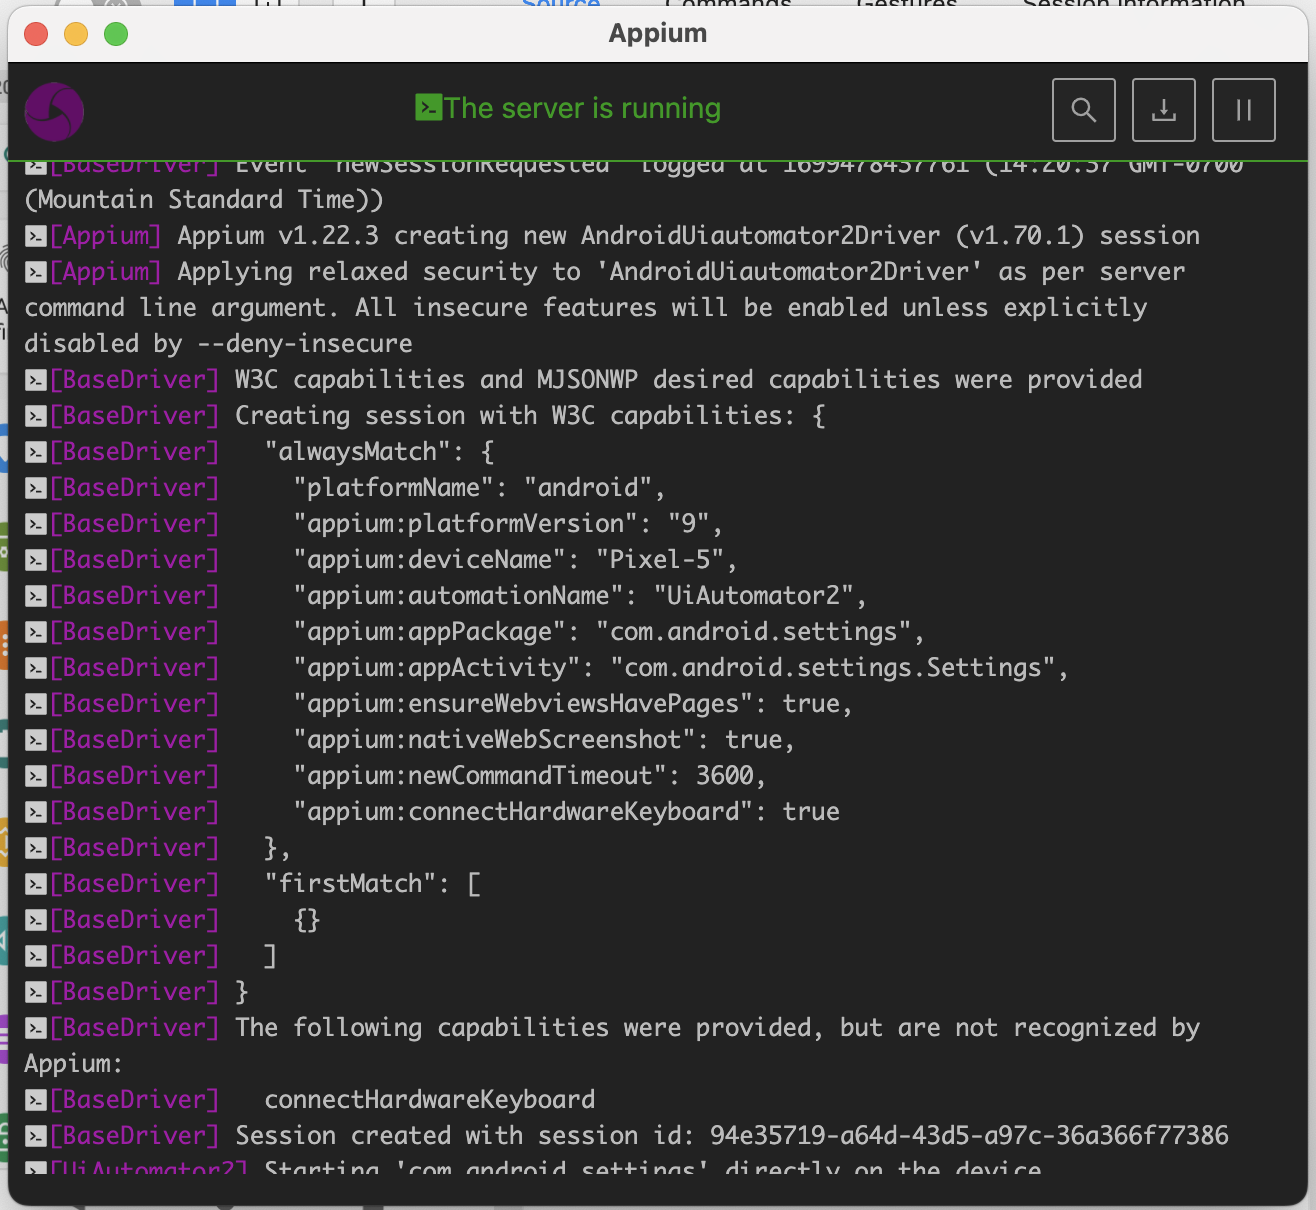
\includegraphics[scale=0.5]{graphics/appium-server.png}
    \caption{Successful Server Connection}
    \label{fig:appium-server}
\end{figure}

\bigskip
\begin{mdframed}[backgroundcolor=blue!10,style=code,nobreak=true,align=center,userdefinedwidth=14cm]
\textbf{Action}
\bigskip

2.2.1 - Connect to the device with the correct parameters and submit a screenshot of your Appium server log reading to you the successful connection.
\end{mdframed}

Once you have successfully connected, Appium will open the inspector and provide you a view of the target application and the page you are trying to copy. In the viewport on the left, you are able to interact with the application as if it were a normal emulator, toggling between different pages and buttons. This allows you to navigate throughout the application and explore the layouts of each different one. Ideally, you’ll want to stay on the page you targeted and inspect the elements within the page. As you can see on the right side of the GUI, you will have an XML layout of the application that serves as a framework for you to recreate the UI of the target application. Furthermore, this is where you will want to take a screenshot of the target application to mimic the background. Some elements will need to be added, as required by Android Studio, such as layoutWidth and layoutHeight. Though you need to add certain elements to make this compatible within Android Studio, it provides a quick and easy method that gives every element within the screen. This will serve as your malicious application in order to trick an unsuspecting user.

\bigskip
\begin{mdframed}[backgroundcolor=blue!10,style=code,nobreak=true,align=center,userdefinedwidth=14cm]
\textbf{Action}
\bigskip

2.2.2 - Inspect the layout of your target application. What is the layout of your file? Submit a screenshot.
\end{mdframed}

\begin{figure}[!h]
    \centering
    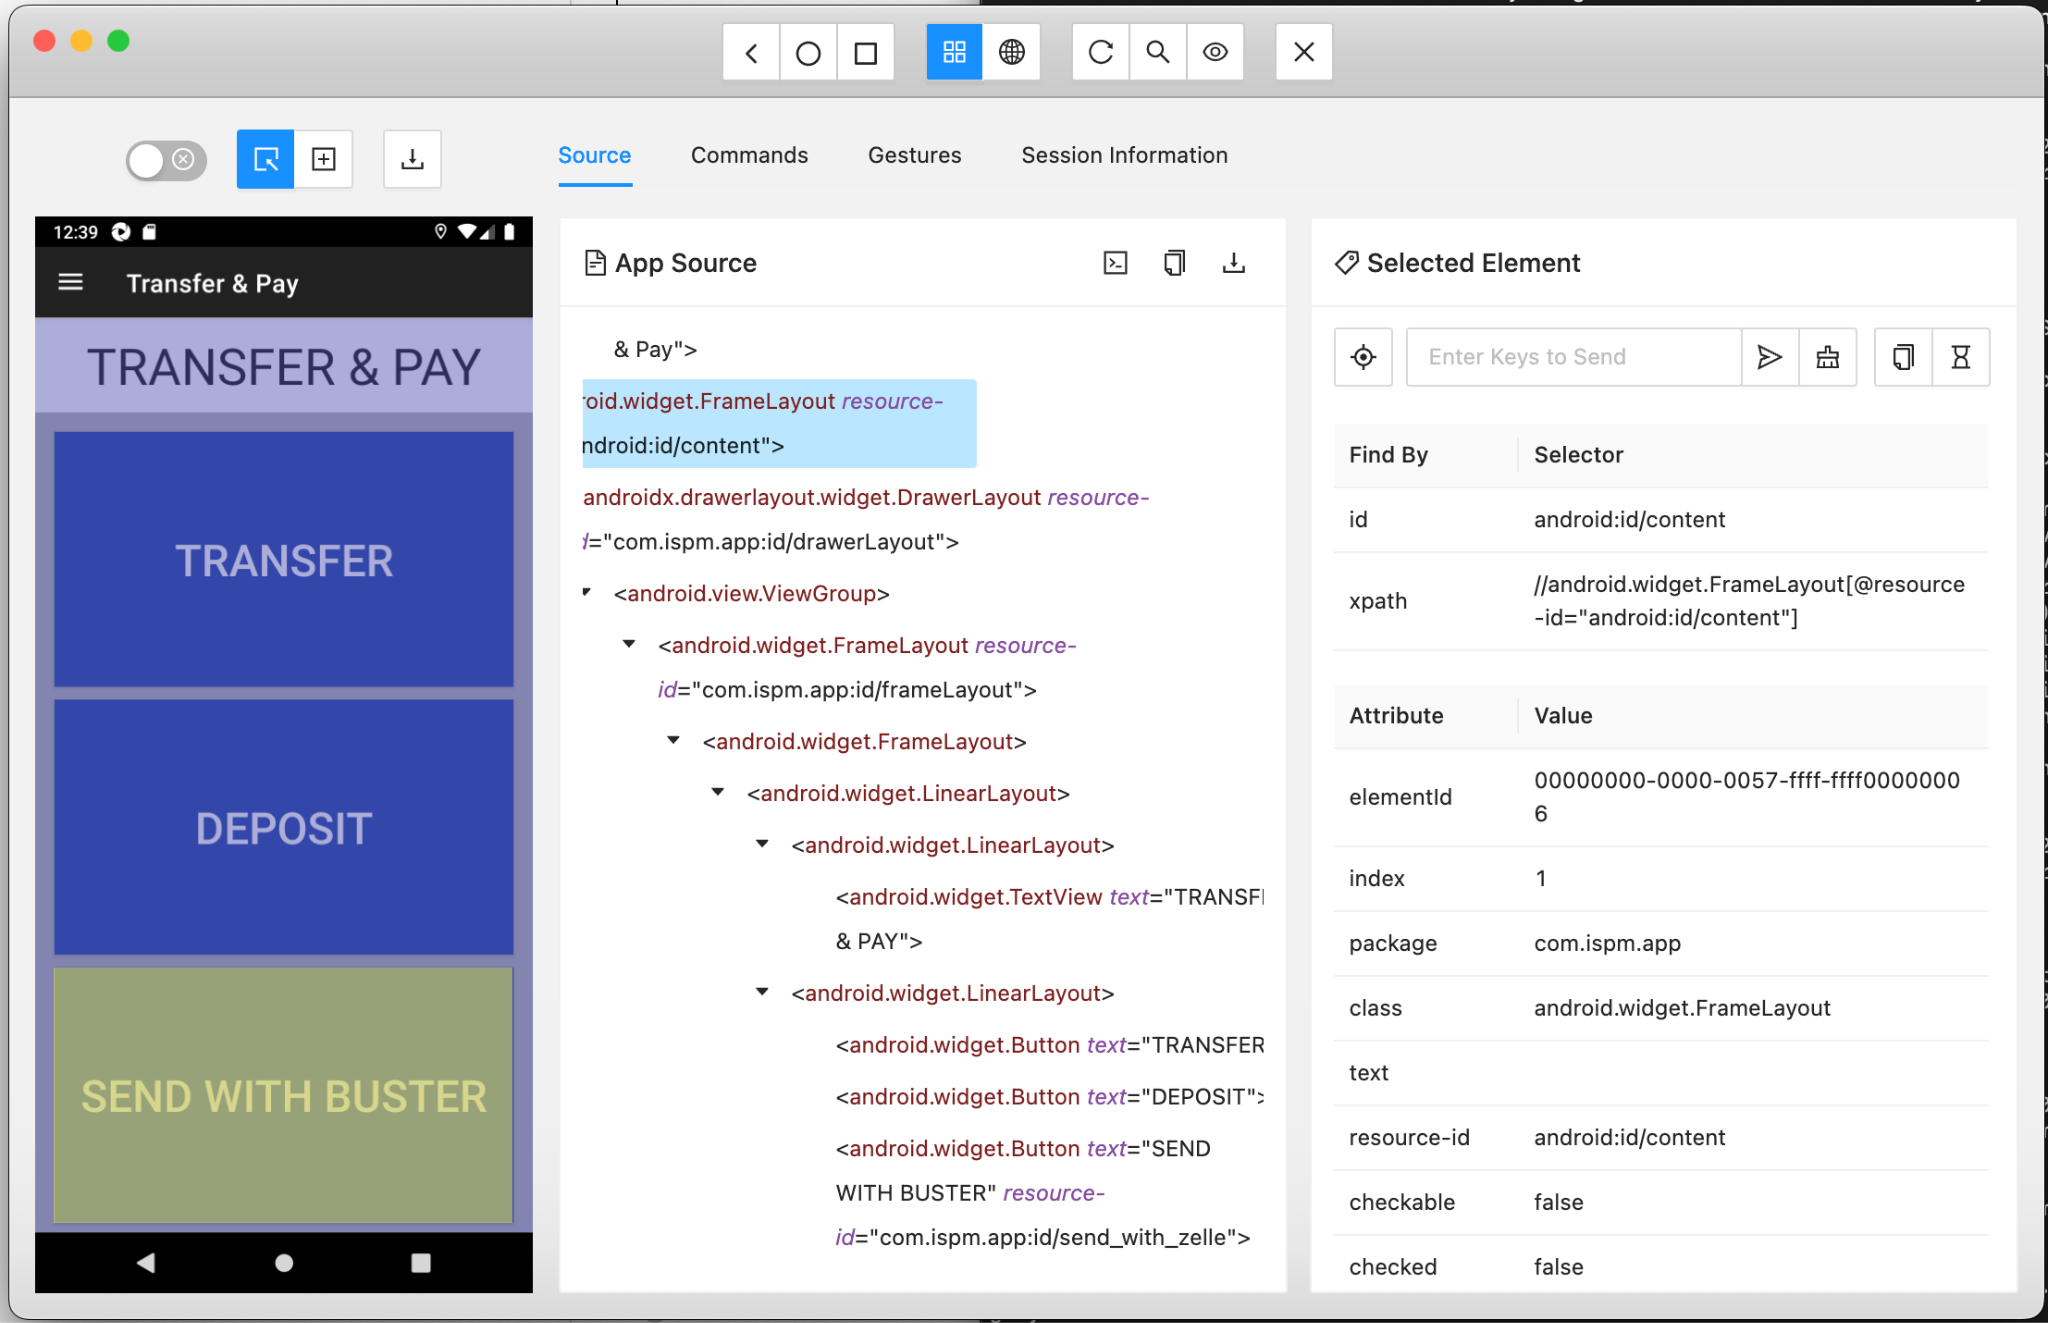
\includegraphics[scale=0.175]{graphics/appium-inspector.png}
    \caption{Inspecting Application}
    \label{fig:appium-inspector}
\end{figure}

\textit{Note:} If you receive an error where the inspector reads “Could not obtain screenshot: Unable to capture the screen”, navigate to your terminal and run the command:

“adb root”. This will provide you root access and remove the security flag that causes this issue.

\subsection*{Task 2.3 Generating Fake UI \& Patchfile}
\addcontentsline{toc}{subsection}{Task 2.3 Generating Fake UI \& Patchfile}

Many apps today use hot patch frameworks that allow patch files to be sent over a server and installed directly to the application. An example of this framework that was explored within the research paper was Tinker. In our exploration, we will be using the Android Studio’s built in functionality that permits us the ability to create and apply them more easily. While we will not be sending this patch over a network and applying it remotely, it is important to understand the process to successfully mimic the attack. 
		
Copy the XML file generated from the Appium Inspector and import it into the AndroidLayout.xml file. Here is where you will make your respective changes to make the XML compatible with Android Studio’s format. After making a few additions and changes, your malicious activity should now very closely resemble the target application you chose to attack. 

\bigskip
\begin{mdframed}[backgroundcolor=blue!10,style=code,nobreak=true,align=center,userdefinedwidth=14cm]
\textbf{Action}
\bigskip

2.3.1 - Take a screenshot of the target application on Appium. Use this as the target image for the layout in Android Studio. Submit a screenshot of both your malicious activity and of the target activity that was replicated.
\end{mdframed}

Now that you have successfully mimic’d the target application, it is time to generate your patch file. On mobile devices, patch files do not re-install class files (such as java or kotlin). Instead, they reinstall the library and dependency files, such as your XML layout, your manifest files, or your build packs. This feature is what makes it possible for us to create a completely fake application that updates and adapts without the need for reinstallation or redistribution. Within Android Studio, stage your changes to the activity\_main.xml file--but \textbf{DO NOT} commit your changes--in your view finder, navigate to Git -> Patch -> Create Patch from Local Changes and select the xml file that you staged.

\bigskip
\begin{mdframed}[backgroundcolor=blue!10,style=code,nobreak=true,align=center,userdefinedwidth=14cm]
\textbf{Action}
\bigskip

2.3.2 - Generate a patch file with your newly updated XML layout for your application and submit a screenshot of both the successful alert message along with the generated layout.
\end{mdframed}

\begin{figure}[!h]
    \centering
    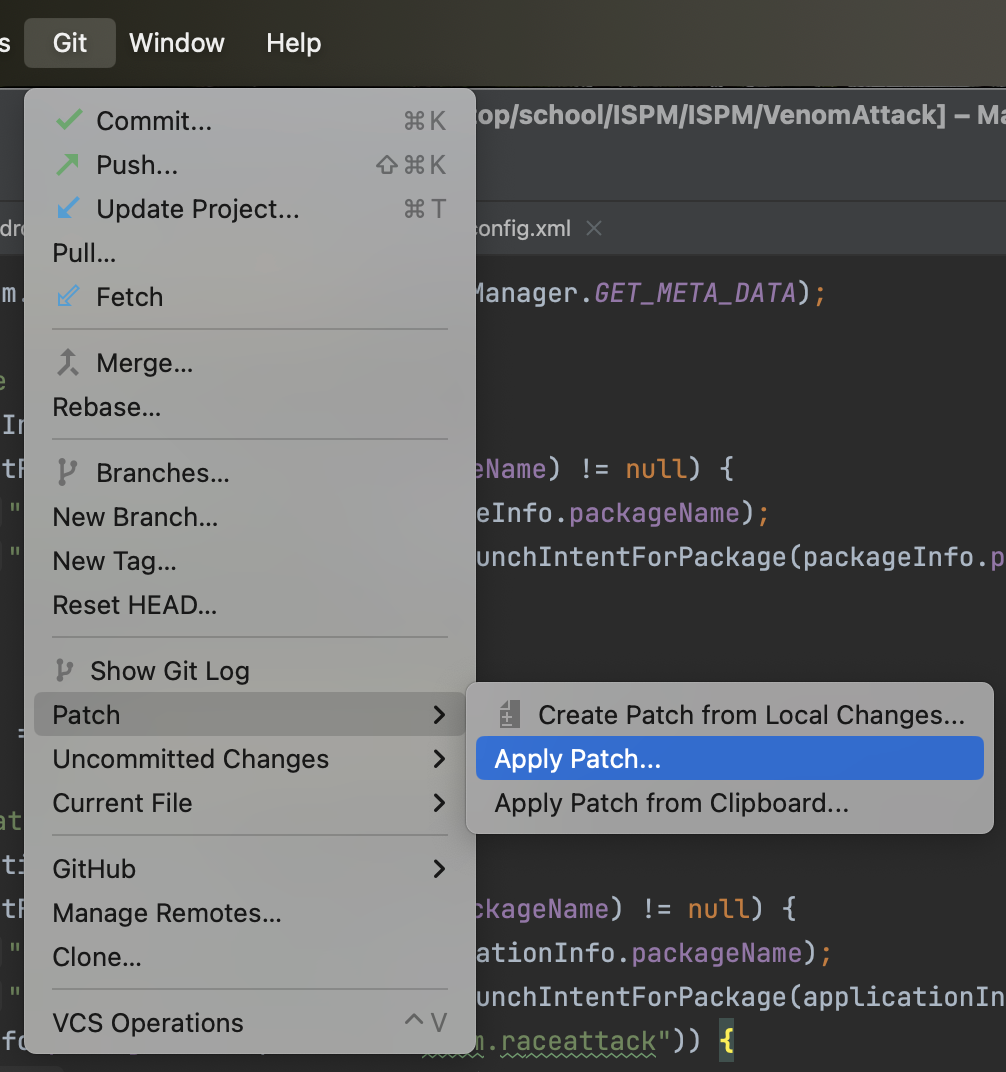
\includegraphics[scale=0.45]{graphics/patch.png}
    \caption{How to Generate a Patch}
    \label{fig:patch}
\end{figure}

%%%%%%%%%%%%%%%%%%%%%%%%%%%%%%%%%%%%%%%%%
%%% Lab Task 3
%%%%%%%%%%%%%%%%%%%%%%%%%%%%%%%%%%%%%%%%%

\section*{Task Set 3: Game Theory}\label{sec:Task 3: Game Theory}
\vspace{-0.35cm}
{\footnotesize Video: \href{https://www.youtube.com/watch?v=nY5Gc6RURes}{\emph{The Purification Theorem}}}
\addcontentsline{toc}{section}{Task Set 3: Game Theory}
\bigskip

In this task set, we are going to explore two game theory concepts: cutpoint strategies and the purification theorem. This will utilize some basic statistical knowledge such as probability and cumulative density functions. 

In a game of cutpoint strategies, there is a continuum of possible types, where some action could cost anything between a lower bound and an upper bound. The information is incomplete, as each player's cost is private information. A cutpoint equilibrium helps us identify what every type of player will do. This cutpoint follows the rule that all types below a cutpoint take one action and all types above it take the opposite action. 

\begin{figure}[!h]
    \centering
    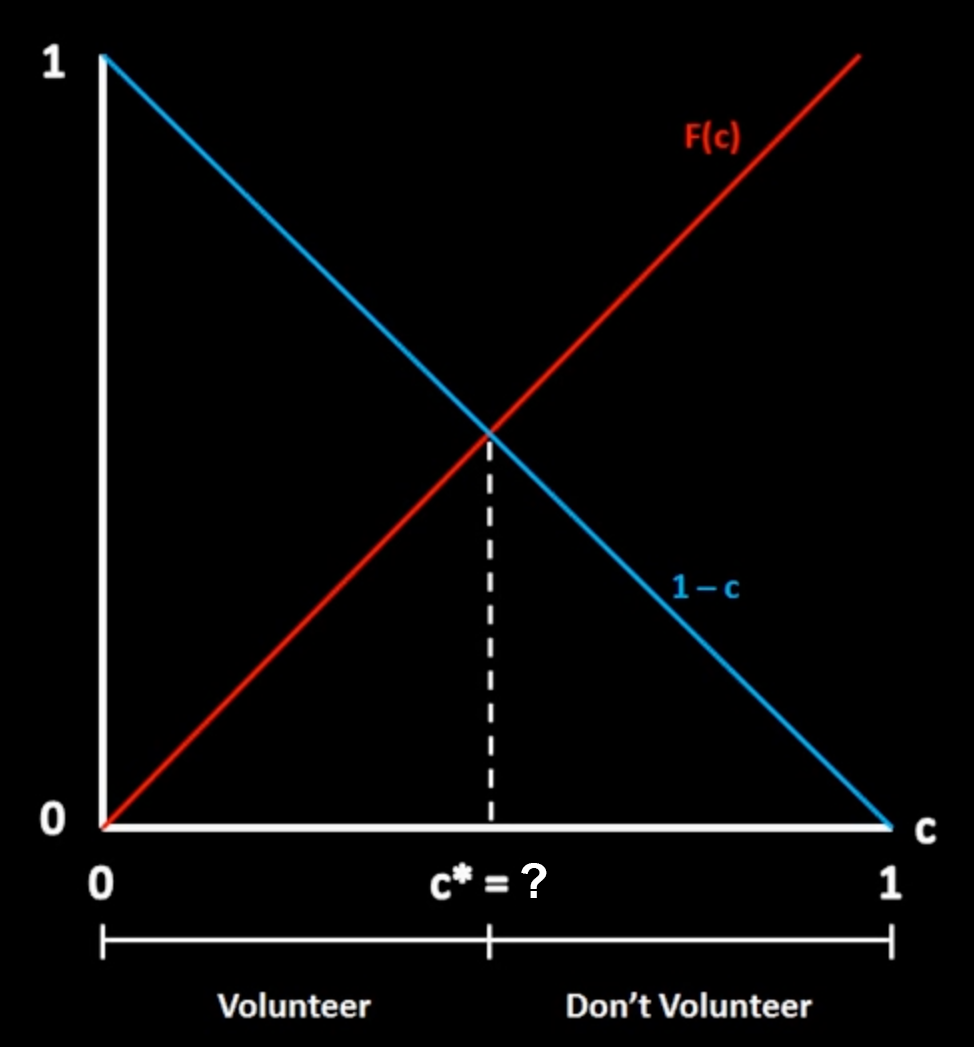
\includegraphics[scale=0.25]{graphics/gt-cstar.png}
    \caption{Continuous Cutpoint CDF}
    \label{fig:gt-cstar.png}
\end{figure}
\bigskip

\bigskip
\begin{mdframed}[backgroundcolor=blue!10,style=code,nobreak=true,align=center,userdefinedwidth=14cm]
\textbf{Action}
\bigskip

3.1.1 - If we were to consider the CDF independently drawn in Figure~\ref{fig:gt-cstar.png} from a symmetric cumulative distribution that is continuous and strictly increasing, what would the cutpoint (c*) be equal to?
\end{mdframed}

\begin{figure}[!h]
    \centering
    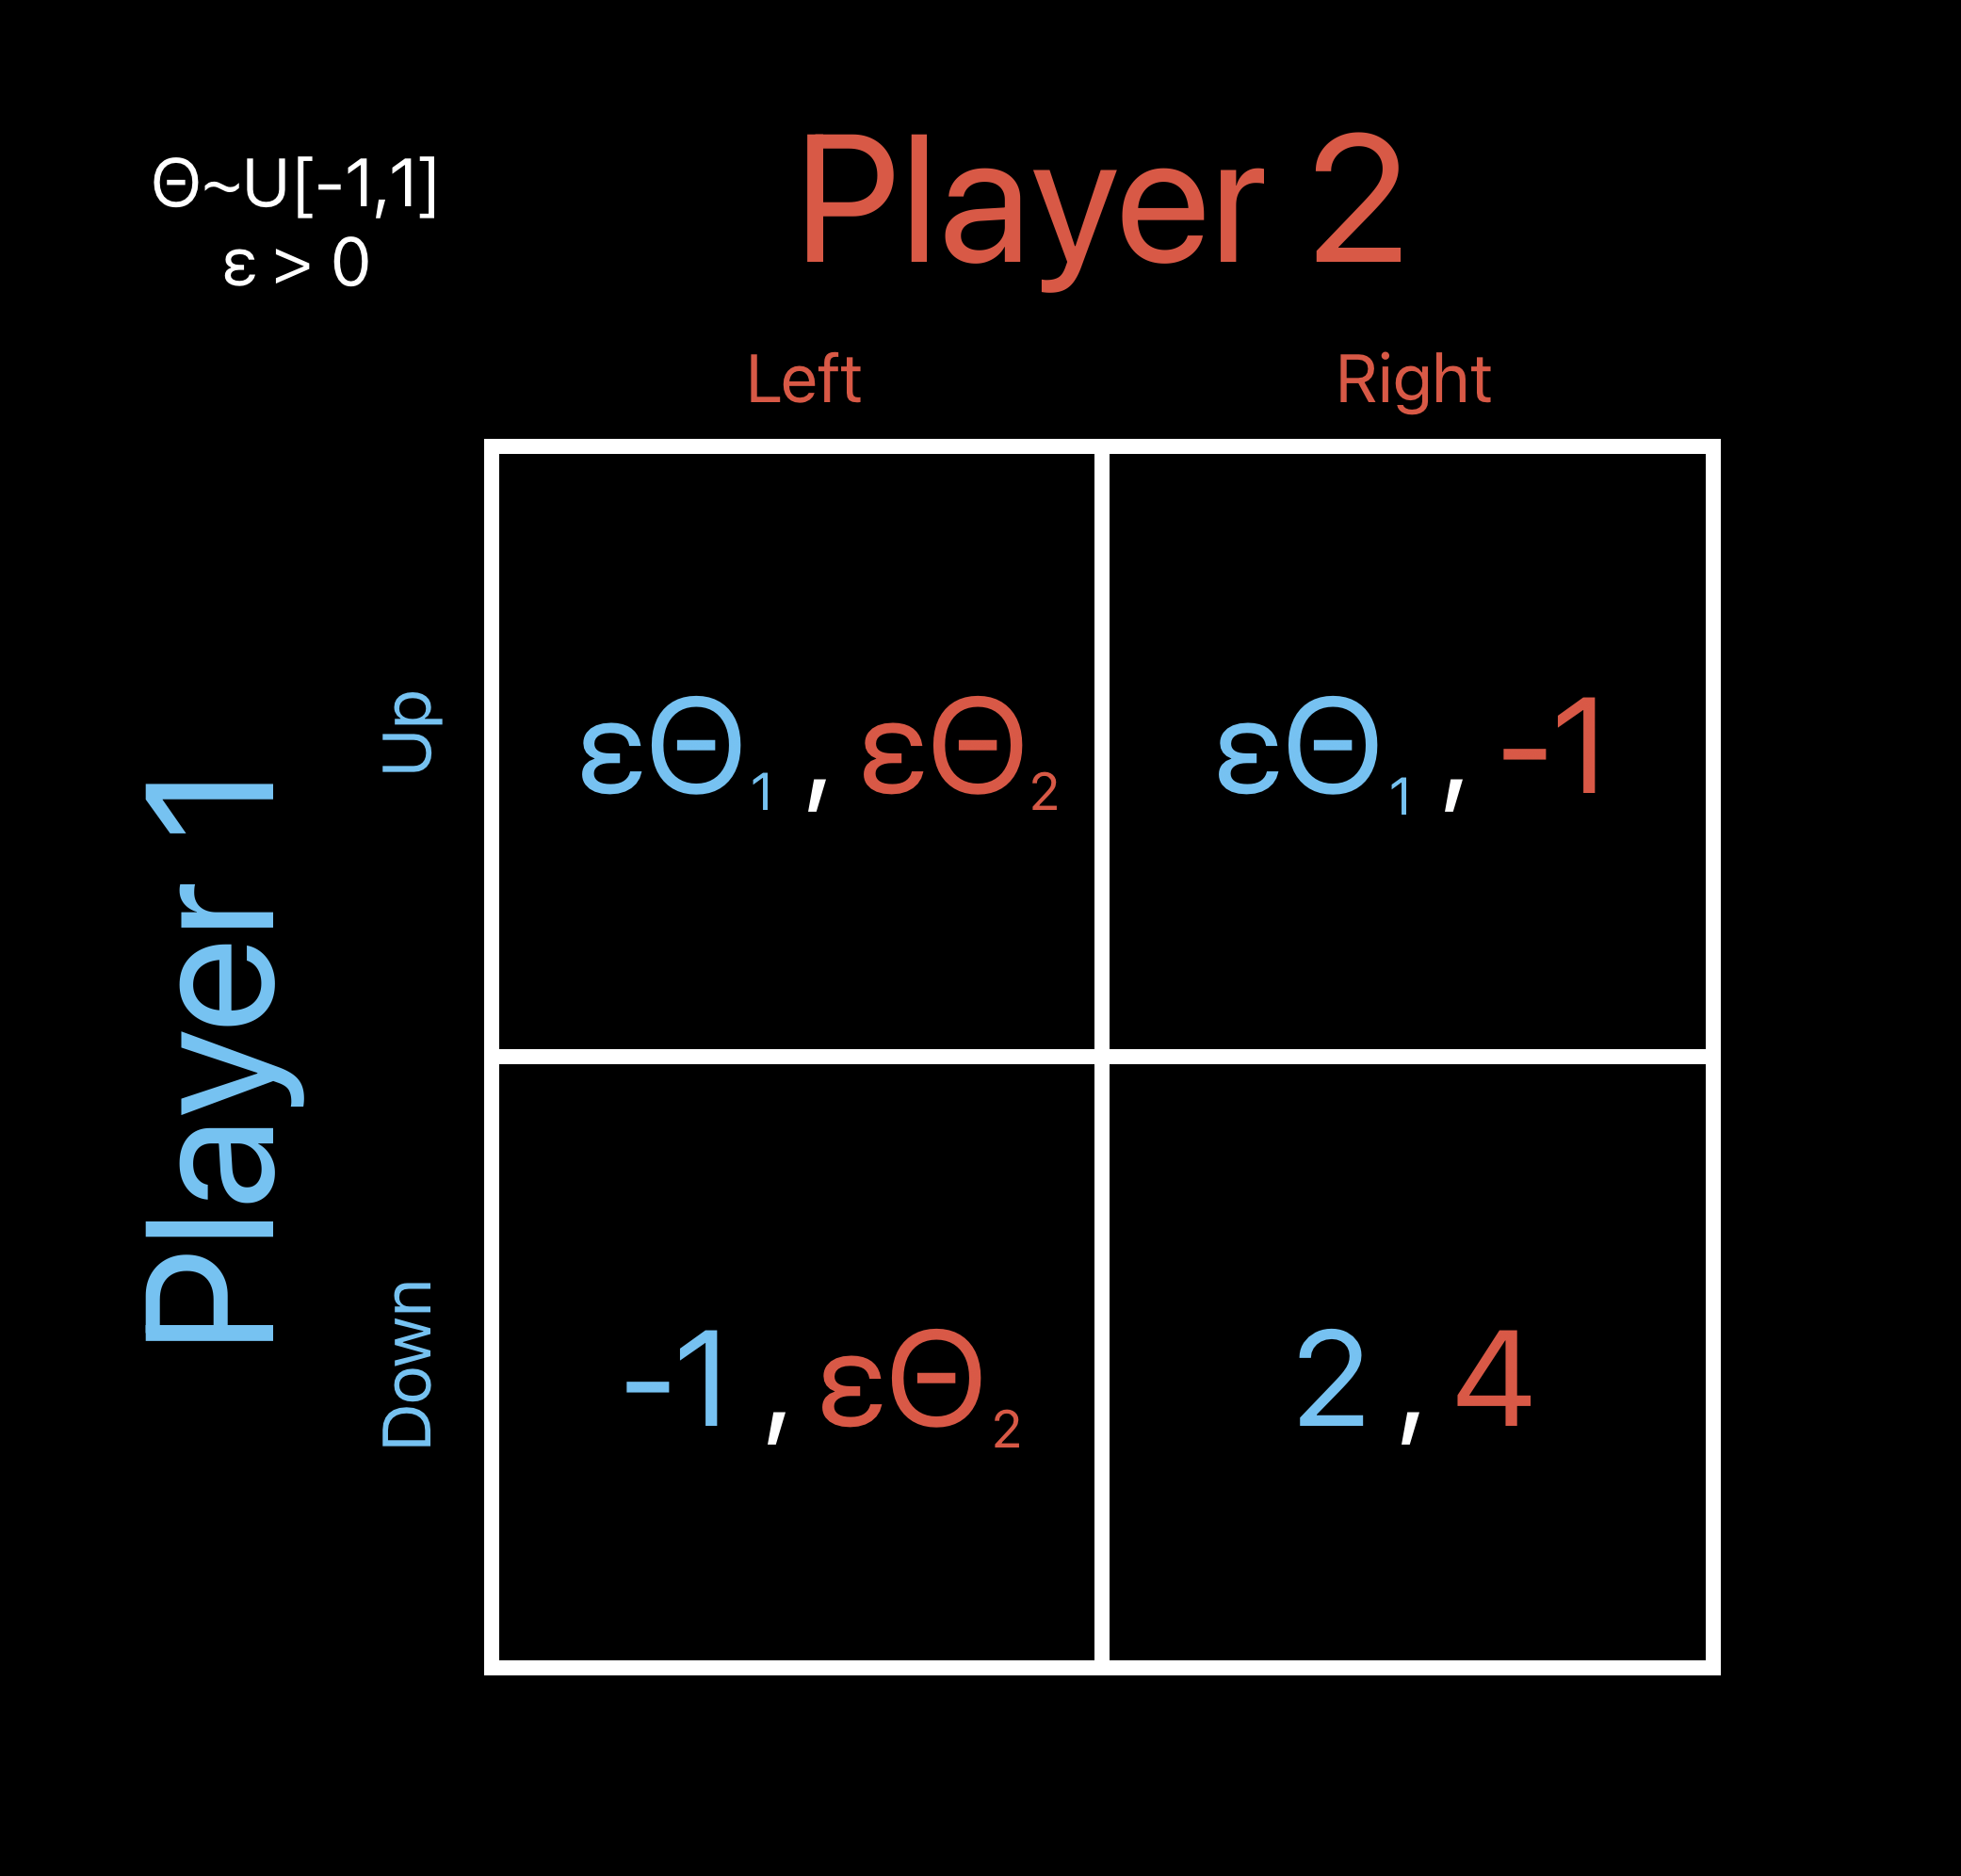
\includegraphics[scale=0.25]{graphics/gt-table.png}
    \caption{Game Theory Table}
    \label{fig:gt-table.png}
\end{figure}
\bigskip

Now lets calculate the cutpoint equilibrium using the table descried in Figure~\ref{fig:gt-table.png}. To start off, we need to calculate each players cutpoint equation.

\textbf{Player 1's Cutpoint:}

$$ \varepsilon\Theta_{1} > p(-1) + (1 - p)(2) $$
$$\Theta_{1} > \frac{(2 - 3p)}{\varepsilon} $$

The system of equations above represents the probability equation that player 1 will play up given the probability, $p$, that player 2 plays left. Now let's calculate player 2's cutpoint. 

\textbf{Player 2's Cutpoint:}
$$\varepsilon\Theta_{2} > q(-1) + (1 - q)(4) $$
$$\Theta_{2} > \frac{(4 - 5q)}{\varepsilon} $$

This will be the probability equation that player 2 will play left given player 1's probability, $q$, that player 1 plays up. Now let's recall from basic probability theory that if $\Theta$ is distributed uniformly from -1 to 1, then the probability that drawing a value smaller than $x$ is:

$$ \frac{x + 1}{2} $$

Therefore the probability of drawing a value of $\Theta_{1}$ greater than $x$ is:

$$ 1 - \frac{x + 1}{2} $$

This is just essentially writing out the cumulative distribution function. If you were to plug $-1$ into the first equation, you would expect a probability of $0$, as $-1$ is the lower bound of the distribution. If you were to plug in $1$, it is the upper bound of the distribution and you are guaranteed to draw something less than it, thus your output would be $1$. 

In order for us to calculate the cutpoint equilibrium, we need to find our probabilities, $p$ and $q$. In order to do this, we first must calculate our system of equations for $p$ and $q$ by substituting the inequality derived in the previous parts for $x$ in the cumulative distribution function. 

\bigskip
\begin{mdframed}[backgroundcolor=blue!10,style=code,nobreak=true,align=center,userdefinedwidth=14cm]
\textbf{Action}
\bigskip

3.1.2 - Substitute each inequality in for x and derive the system of equations for both p and q. What are these equations?

\bigskip

\emph{Hint: Set one of the variables equal to the cumulative distribution function and substitute the opposing variable in for $x$.}
\end{mdframed}

Now that you have your system of equations, we can solve for the probabilities $p$ and $q$. Substitute the equation for one probability into the respective probability of the other equation and vice-versa. You should be left with two final equations, with the only unknown variable being $\varepsilon$. If you recall, $\varepsilon$ is a number that is greater than but converging to $0$. 

\bigskip
\begin{mdframed}[backgroundcolor=blue!10,style=code,nobreak=true,align=center,userdefinedwidth=14cm]
\textbf{Action}
\bigskip

3.1.3 - Substitute $0$ in for $\varepsilon$ to calculate the probabilities for both $p$ and $q$. What are the probabilities of $p$ and $q$?
\end{mdframed}

These two values are your cutpoint equlibria. As this game converges from an incomplete information game to a complete information game, then the equilibrium probabilities of the players taking particular actions exactly match the probabilities from the complete information games mixed strategy nash equilibrium.

%%%%%%%%%%%%%%%%%%%%%%%%%%%%%%%%%%%%%%%%%
%%% Submission
%%%%%%%%%%%%%%%%%%%%%%%%%%%%%%%%%%%%%%%%%

\section*{Submission}\label{sec:Submission}
\addcontentsline{toc}{section}{Submission}

Submit a lab report utilizing the provided template to your instructor, which should include screenshots, thoughts, challenges, and lessons learned from the lab. Furthermore, zip and attach your project files with the relevant java files for submission.

%%%%%%%%%%%%%%%%%%%%%%%%%%%%%%%%%%%%%%%%%
%%% Summary
%%%%%%%%%%%%%%%%%%%%%%%%%%%%%%%%%%%%%%%%%

\section*{Summary}\label{sec:Summary}
\addcontentsline{toc}{section}{Summary}

In this lab we've discovered how to gather information from an Android app and send it to a remote server, in our case a NodeJS Express server, utilize Appium to automatically generate UI layouts, and how to create a patch file to update an application without needing to reinstall it. All together, these methods allow attackers to be able to update attack payloads without the need for re-installation or redistribution, further increasing the impact of activity hijack attacks.

\section*{Trouble Shooting}\label{sec:Trouble Shooting}
\addcontentsline{toc}{section}{Trouble Shooting}

\subsection*{Refactoring the Project Name}\label{sec:Refactoring-the-Project-Name}
\addcontentsline{toc}{subsection}{Refactoring the Project Name}

• Make sure you change the respective lines within build.gradle and AndroidManifest.xml to match what you refactored your project to. Then, select File -> Invalidate Caches -> Restart, and your project should rebuild with the correct dependencies. If this does not work, you can select Build -> Clean Project and Build -> Rebuild Project and then retry invalidating the caches. This should fully correct your problem.

\bibliography{References}
\bibliographystyle{plain}

\end{document}

%%%%%%%%%%%%%%%%%%%%%%%%%%%%%%%%%%%%%%%%%